\section{Introduction and construction}\label{dec:introduction}

\begin{quote}
{\small We introduce the main objects of study and briefly describe the construction of the corresponding stochastic processes. The construction gives rise to important properties that we discuss. }
\end{quote}

\subsection{Introduction}\label{ssec:introduction}
The East model is an interacting particle system evolving with a Glauber like dynamics on the state space $\Omega \defeq \{0,1\}^\Z$. It belongs to a class of stochastic processes called kinetically constrained spin models (KCMs), with the East model being the first of these to be studied rigorously. The process evolves as follows: at each site $x \in \Z$ the system tries to update the value of the spin at $x$ to 1 or 0 at rate $p \in (0,1)$ and $q \defeq 1 - p$ respectively. The update is accepted only if a local constraint is satisfied, which in the East model's case is that the occupation variable at site $x-1$ must be equal to 1. Sometimes we will call elements of $\Omega$ \textit{configurations} and say a site is \textit{occupied} or \textit{infected} if its spin value is equal to 1. \\

In the sections to follow we focus on two objects of interest related to the East model. The first one is the speed of the so-called \textit{front}. Consider an East model started from the configuration equal to all 0 except at the origin. It is easy to see that the spins on $(-\infty, 0]$ stay frozen for all time, and infection 'spreads' to the right. A natural question to ask then is how fast this spreading of infection happens \textit{if} it happens at all. We define the front to be the rightmost infected site in the configuration at time $t$. In our study of the speed of the front we will compare the East model to a second stochastic process called the one-sided contact process. The one-sided contact process has the same state space $\Omega$ and evolves as follows: each site \textit{recovers} i.e. sets its spin to 0 at rate $q$ and gets infected by its left neighbour (provided the neighbour is infected) at rate $p$. The second object of interest is the \textit{mixing time} of the East process when restricted to $\{ 0, 1, ..., L\}$ for some $L \in \N^+$. We will study the mixing time for the East model on $\{ 0, 1, ..., L\}$ with the occupation variable of the origin fixed to be $1$, so that the evolution at site 1 is unconstrained. \\

The main results of this paper can be summarised as follows. We show that for $p$ larger than a critical value the front of the East model started from exactly one infection propagates at precisely linear speed. We also show that for such $p$ the mixing time on $\{ 0, 1, ..., L\}$ is $\Theta(L)$\footnote{We say $f = \Theta(g)$ if there exist constants $K_1, K_2$ such that for all large enough $n \in \N$ it holds that $K_1 g(n) \leq f(n) \leq K_2 g(n)$.}. In the process of proving these we show exponential bounds on the front propagation and survival time of the one-sided contact process. The results concerning the East model have been known to hold under weaker restrictions on $p$ for some time, see \cite{ganguly2015cutoff} for a review. The results concerning the one-sided contact process were first stated in \cite{durrett1983supercritical}, but to our knowledge never proved in detail. The paper is broken into 5 chapters. The second chapter contains the statements of our main results. Chapter three discusses the one-sided contact process and presents proofs of the above mentioned exponential bounds. Chapter four is devoted to the proof of Theorem \ref{main_thm:speed} while in chapter five we present the proof of Theorem \ref{main_thm:mixing}. 


\subsection{Constructing the basic coupling}
Let $\scr{C} = (E_{x,k}, B_{x,k})_{x \in \Z, k \in \N^+}$ be a collection of independent random variables with $E_{x,k} \sim \dExp{1}$ and $B_{x,k} \sim \dBer{p=1-q}$. Define the times 
\[
T_{x,n} \defeq \sum\limits_{k=1}^n E_{x,k}
\]
 also referred to as \textit{clock rings} and call a clock ring $T_{x,n}$ \textit{legal} if the local constraint of the corresponding process is satisified at site $x$ at time $T_{x,n}$. We can now construct the East model $(\sigma_t)_{t \geq 0}$ and the one-sided contact process $(\eta_t)_{t \geq 0}$ using $\scr{C}$ as follows. 
 
For each site $x \in \Z$ at each time $T_{x,n}$:
\begin{itemize}
  \item If $B_{x,n} = 1$:
  \begin{enumerate}
  	\item If $\sigma_{T^-_{x,n}} (x-1) = 1$ update $\sigma$ to 1 at site $x$. 
  	\item If $\eta_{T^-_{x,n}} (x-1) = 1$ update $\eta$ to 1 at site $x$. 
  \end{enumerate}
  \item Else:
  \begin{enumerate}
  	\item If $\sigma_{T^-_{x,n}} (x-1) = 1$ update $\sigma$ to 0 at site $x$. 
  	\item Update $\eta$ to 0 at site $x$. 
  \end{enumerate}
\end{itemize}

\begin{figure}[!h]
  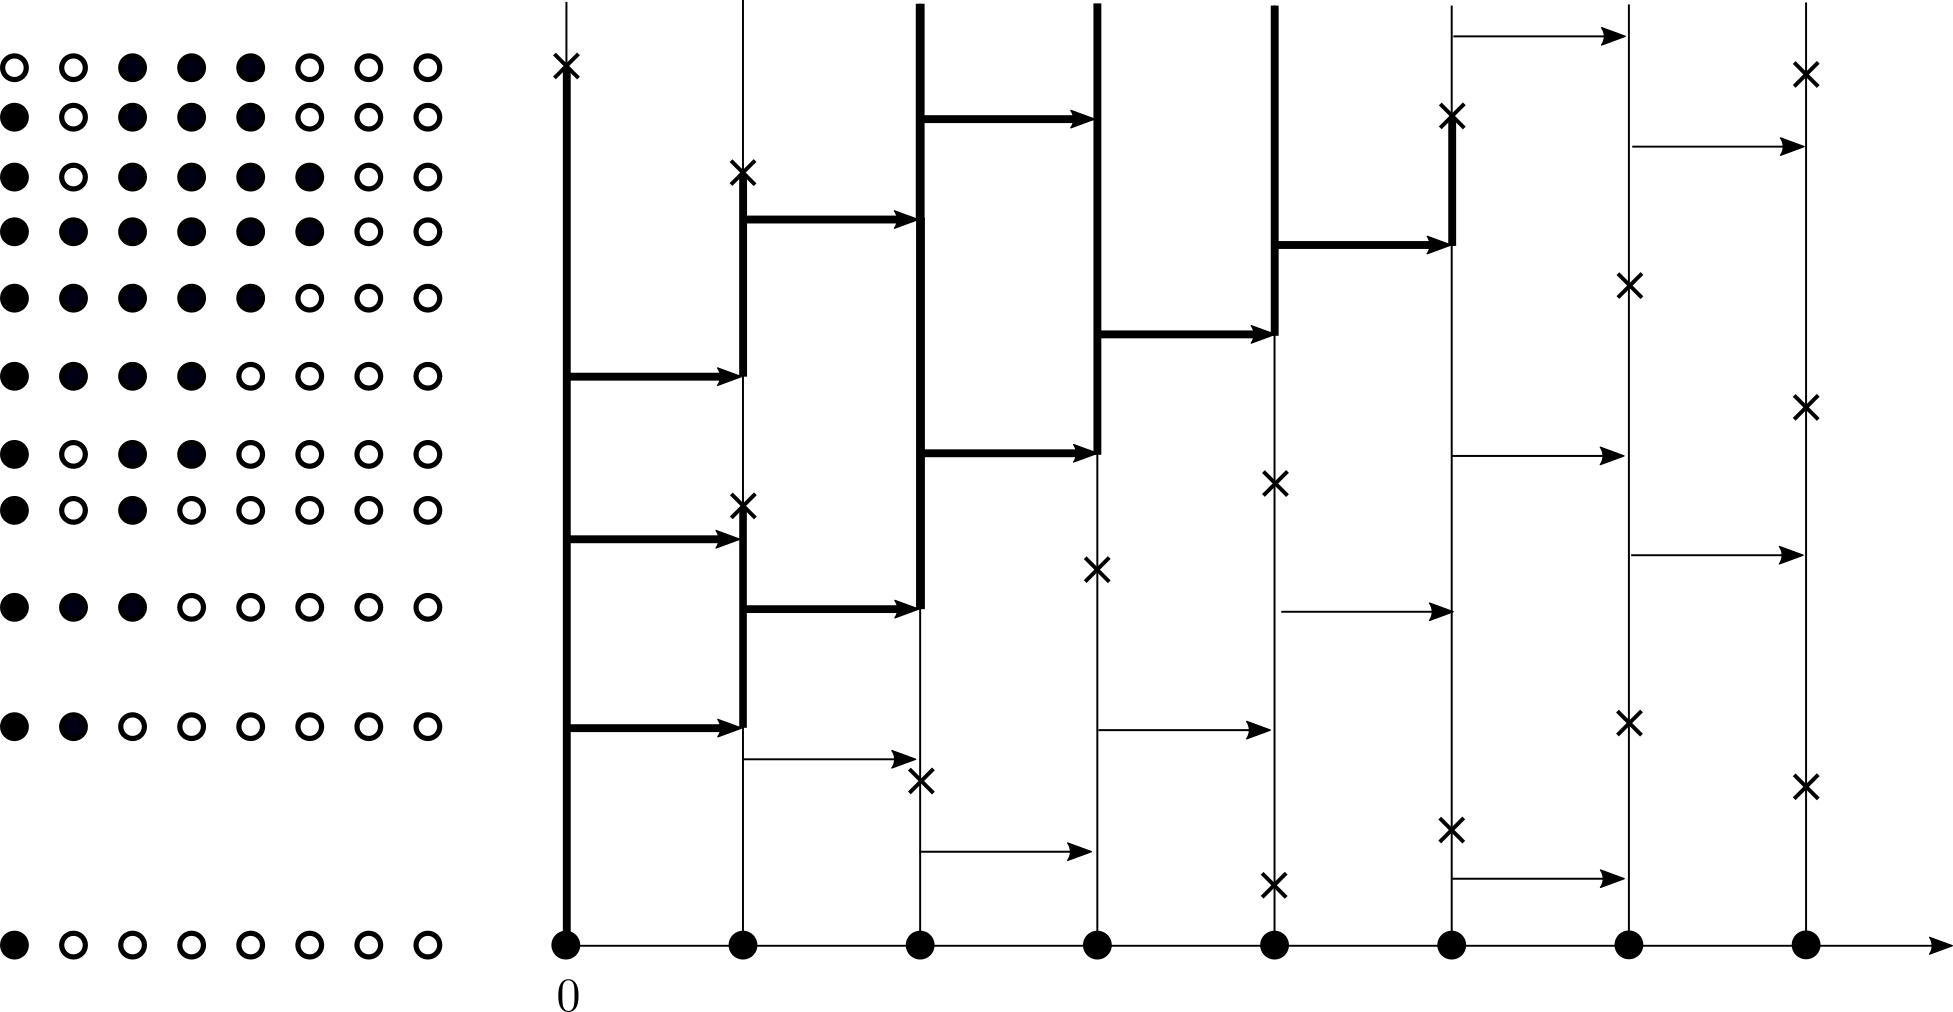
\includegraphics[width=\linewidth]{graphical_construction}
  \caption{Harris' graphical representation, showing the evolution of a one-sided contact process started from site $0$. }
  \label{fig:graphical_construction}
\end{figure}

There is a graphical representation of $\scr{C}$ introduced by Harris that is a helpful tool for visualizing the evolution of the two coupled processes however we will only use it to analyze the one-sided contact process. We will use the symbol $\scr{P}$ to refer to this graphical construction which we informally describe as follows. First draw vertical lines from $0$ to infinity at each integer in $\Z$. At each site $x \in \Z$ put a cross on the line at $(x, T_{x,n})$ if $B_{x,n} = 0$. If $B_{x,n} = 1$ instead of a cross draw an arrow from $(x - 1, T_{x,n})$ to $(x, T_{x,n})$. Crosses represent recovery while arrows represent infection spreading towards the right. For an example of the graphical representation see Figure \ref{fig:graphical_construction}. 

\begin{notation}[Initial configurations]
Suppose we start a stochastic process $(\xi_t)_{t \geq 0}$ with state space $\Omega$ from initial configuration $\zeta \in \Omega$. The resulting process will be denoted $(\xi^\zeta_t)_{t \geq 0}$. If $\nu$ is a probability distribution on $\Omega$, then we write $(\xi^\nu_t)_{t \geq 0}$ for the process started from a \textit{random} distribution drawn from $\nu$. The initial distribution is drawn independently from $\scr{C}$
\end{notation}
\begin{notation}[$\Omega$ and $\cal{P}(\Z)$]\label{not:powerset}
Because of the natural bijection between the power set of $\Z$ and $\Omega$, we will consider configurations as both subsets of $\Z$ and elements of $\Omega$, regularly switching between the two interpretations. 
\end{notation}

In what follows we only consider contact processes with $\sfrac{p}{q} > \lambda_c$ where $\lambda_c$ is the critical parameter for the one-sided contact process on $\Z$, defined as $\lambda_c \defeq \sup\{ \sfrac{p}{q} : |\eta^{\{0\}}| \rightarrow 0\ a.s.\}$. A one-sided contact process with rates satisfying this condition is called supercritical. By definition the extinction time $\tau(\eta^{\{0\}}_.) \defeq \inf\{t \geq 0 \mid \eta^{\{0\}}_t = \varnothing \}$ of a supercritical one-sided contact process satisfies $\Pr{\tau(\eta^{\{0\}}_.) = \infty} > 0$ i.e. the process survives forever with positive probability. 

\begin{notation}[Supercritical East model]
As per the previous discussion, we call an East model supercritical if $\sfrac{p}{q} > \lambda_c$. 
\end{notation}

\subsection{Domination and other properties}\label{ssec:intro_properties}
The basic coupling has two important properties that follow immediately from its definition. First, it lets us construct both processes started from any initial configuration on the same probability space. The second property is domination: if at some time $t \geq 0$ it holds that $\eta_t \leq \sigma_t$ then $\eta_{t+s} \leq \sigma_{t+s},\ \forall s \geq 0$. To see this note that under the graphical construction $\eta$ updates a particular site to 1 only if $\sigma$ does too, and $\sigma$ updates a particular site to 0 only if $\eta$ does too. In particular, if $X(\cdot)$ denotes the position of the front then $X(\eta_{t+s}) \leq X(\sigma_{t+s}),\ \forall s \geq 0$. \\

Domination is what enables us to bound the East model from below by the one-sided contact process. The reason we might want to do this is that contact processes posess desirable qualities that KCMs in general might not. Contact processes are \textit{attractive} in the sense that if $\nu \subseteq \xi \subseteq \Z$ then $\eta^\nu_t \leq \eta^\xi_t$ for all $t \geq 0$ under the basic coupling. Moreover they are also \textit{additive}: if $\nu, \xi \subseteq \Z$ then $\eta^{\nu \cup \xi}_t = \eta^\nu_t \cup \eta^\xi_t$ for all $t \geq 0$ under the basic coupling. These qualities make contact processes more amenable to analysis than KCMs, and there is a breadth of methods and results already established. The East model lacks both attractivity and additivity, thus the desire to compare it to the `simpler' one-sided contact process is justified. 
